\chapter{Előkészületek és munkamenet}\label{ch:preparation}

\section{A jármű előkészítése}
Kövesse az alábbi lépéseket, amikor a gyári műszeregységet Digifiz műszerfalra cseréli:
\begin{enumerate}
    \item Távolítsa el a pedálokat és az alsó műszerfalat takaró műanyag burkolatot, hogy hozzáférjen a gyári műszeregységhez.
    \item Válassza le az autó akkumulátorát.
    \item Húzza le a kábelkorbács csatlakozóit a gyári műszerről.
    \item Válassza le a mechanikus sebességmérő bowdent, ha van.
    \item Csavarja ki a panelt a konzolból, és óvatosan vegye ki a járműből.
    \item Vezesse el a mellékelt hőmérséklet- és sebességérzékelő kábelkorbácsokat a szükséges módon.
    \item Csúsztassa be a Digifiz műszert a konzol vezetőibe, és rögzítse csavarokkal.
    \item \ReplicaNextLong{} esetén szerelje be a Volkswagen MFA érzékelőket (vagy megfelelőiket), és vezesse a vezetékeiket a CE~1/CE~2 csatlakozókhoz.
    \item A \texttt{GACS}/\texttt{GARS}/\texttt{DARS}/\texttt{DACS} modelleken kézzel kösse be a feliratozott \texttt{MFA\_MODE}, \texttt{MFA\_RESET}, \texttt{MFA\_BLOCK} és kézifék vezetékeket, ha a jármű kábelkorbácsából hiányoznak ezek az érintkezők. A második generációs \ReplicaNextShort{} alapértelmezetten belsőleg kapcsolja ezeket a jeleket.
    \item Csatlakoztassa a kábelkorbácsokat a műszerfalhoz.
    \item Szerelje be az elektronikus sebességérzékelőt, vagy csatlakoztassa vissza a mechanikus bowdent.
    \item Szerelje vissza a műszerfal burkolatait és a pedál takarót fordított sorrendben.
\end{enumerate}

\section{A műszerfal használata}
\begin{itemize}
    \item A műszerfal a gyújtással együtt automatikusan bekapcsol. A helyzetjelző kapcsoló szabályozza a háttérvilágítást.
    \item Indításkor a teljes sebességskála felgyullad, miközben a belső diagnosztika stabilizálja az RPM modellt; ezt követően a kijelző az aktuális alapjáratot mutatja.
    \item Amint a jármű elindul, a rendszer a \Cref{ch:technical-specs} fejezetben felsorolt paramétereket jeleníti meg.
\end{itemize}

\subsection{MFA funkciók}
Hat MFA oldal érhető el:
\begin{enumerate}
    \item Napi üzemidő.
    \item Menettáv.
    \item Üzemanyag-fogyasztás (az első Replica változatban nincs implementálva).
    \item Átlagsebesség (a kijelzett érték tízzel szorozva jelenik meg).
    \item Motorolaj hőmérséklet (külső kábelkorbács szükséges).
    \item Külső hőmérséklet (külső kábelkorbács szükséges).
\end{enumerate}
A \ReplicaGenOneShort{} műszereken a VW embléma mögötti kapacitív érintőpont lépteti az oldalakat; a \ReplicaNextShort{} külső, kormányoszlopra szerelt kapcsolót használ. Az érintési idők viselkedése:
\begin{itemize}
    \item Rövid érintés (\(<1\)~s): a következő MFA funkcióra lép.
    \item Közepes érintés (1--3~s, ha nincs kormánykapcsoló): MFA memória blokkok közötti váltás, amelyet a kijelzőn is jelez.
    \item Hosszú érintés (3--7~s): az aktív MFA funkció nullázása (érinti a fogyasztást, menettávot, eltelt időt és átlagsebességet).
\end{itemize}

\subsection{Háttérvilágítás és visszajelző kiosztás}
A \ReplicaGenOneShort{} műszer kézi fényerő-szabályzót kínál a helyzetjelző kapcsoló felett; a \ReplicaNextShort{} fotodióda által vezérelt automatikus fényerőt használ. Kézi felülvezérlések a \Cref{ch:replica-setup,ch:replica-next-setup} fejezetekben ismertetett karbantartási felületeken állíthatók.

A vízszintes visszajelző blokk elrendezését és a képernyőn megjelenő jelmagyarázatot a \autoref{fig:indicator-layout} ábra mutatja.

\begin{figure}[htbp]
    \centering
    \begin{subfigure}{0.48\textwidth}
        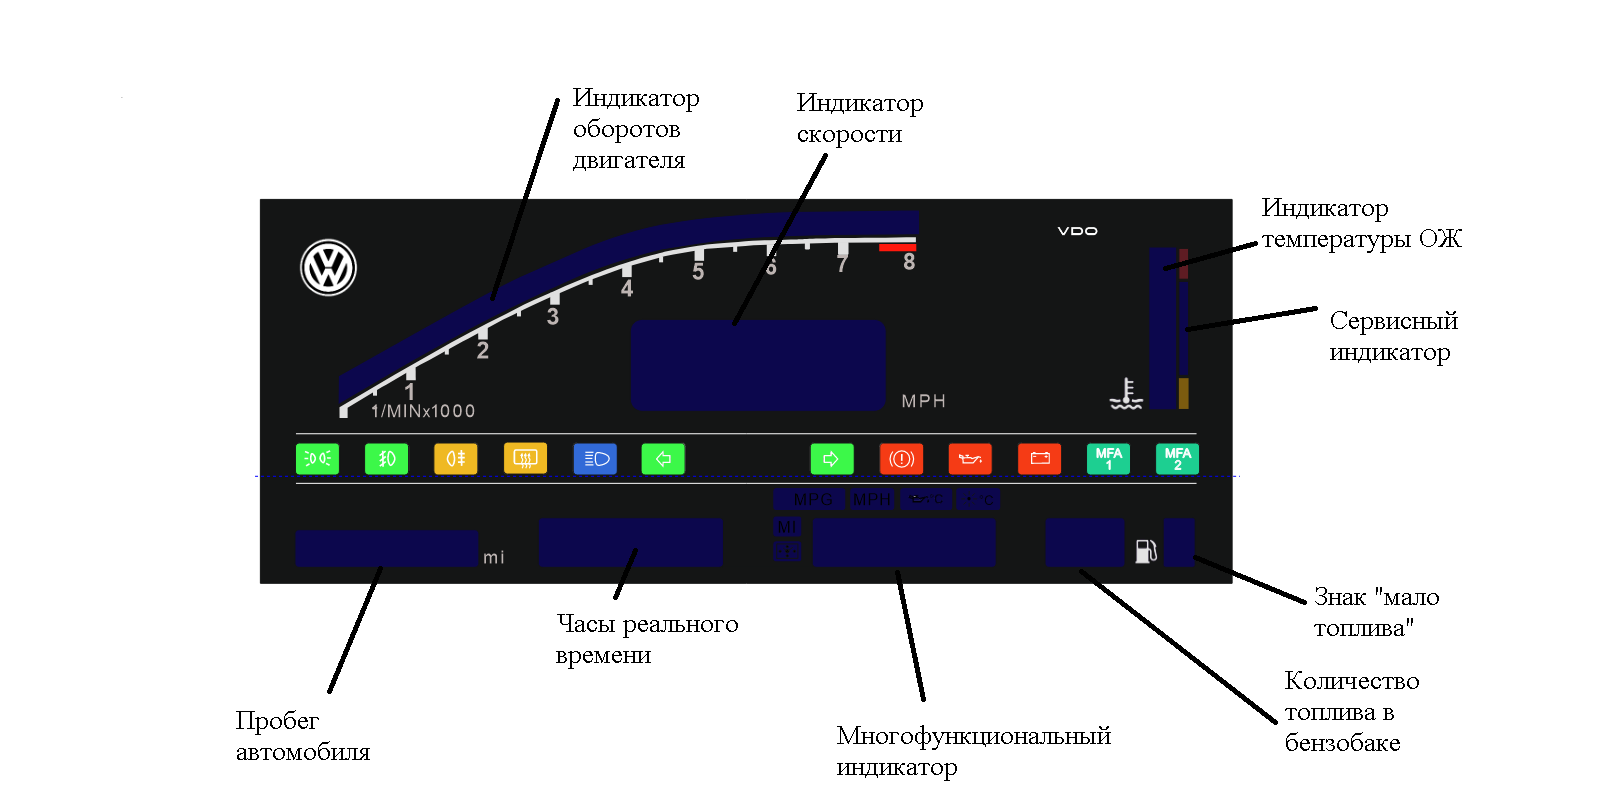
\includegraphics[width=\linewidth]{digifiz_manual/image017.png}
        \caption{Visszajelző elrendezés az indításkori önellenőrzés alatt.}
    \end{subfigure}\hfill
    \begin{subfigure}{0.48\textwidth}
        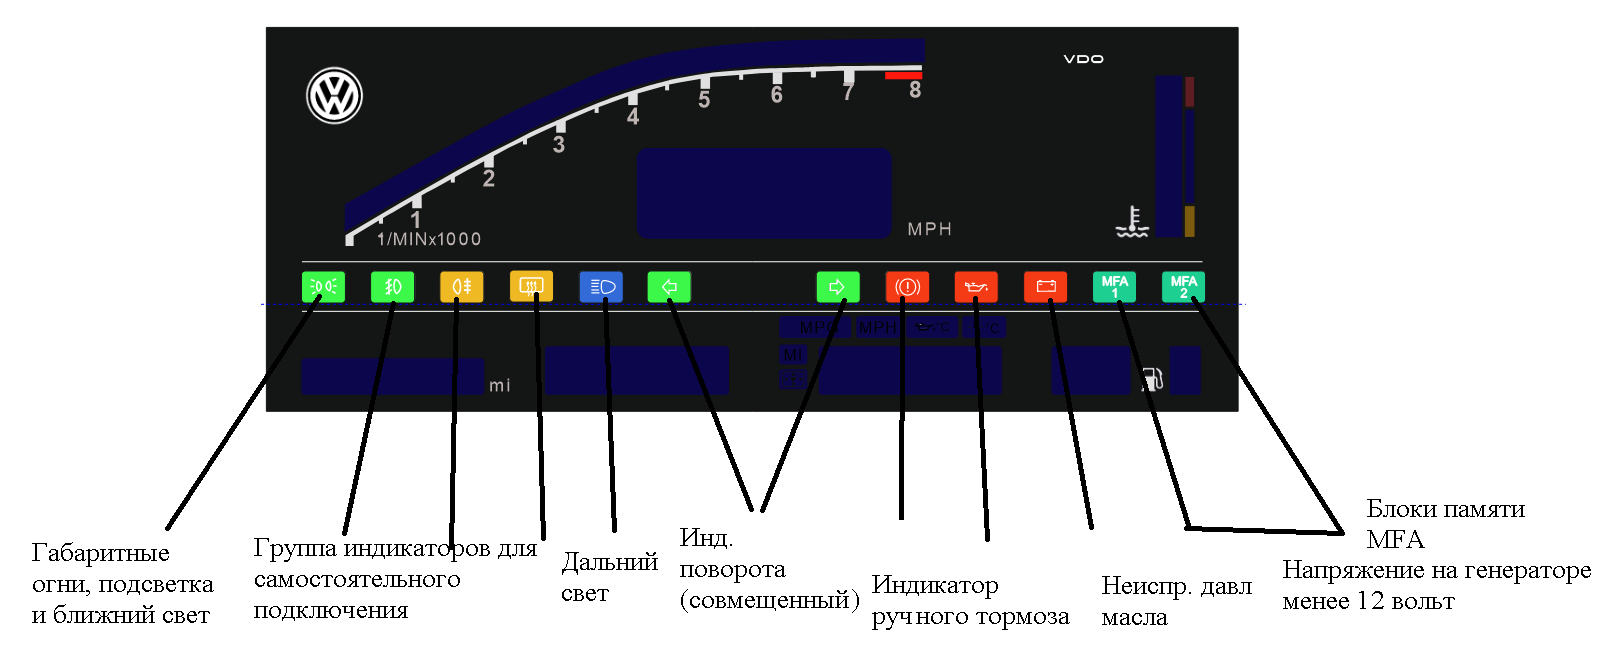
\includegraphics[width=\linewidth]{digifiz_manual/image018.png}
        \caption{A vízszintes visszajelző csoport jelmagyarázata.}
    \end{subfigure}
    \caption{A műszeregység jelzési sémája.}
    \label{fig:indicator-layout}
\end{figure}

\subsection{Konfigurációs felületek}
\begin{itemize}
    \item A klasszikus \ReplicaGenOne{} egységek Bluetooth 2.0 (vagy BLE-kompatibilis) modult tartalmaznak. Telepítse a \emph{Serial Bluetooth Terminal} alkalmazást a Google Play áruházból, párosítsa a műszerrel, és adja ki a parancsokat közvetlenül a terminálnézetből. Apple iOS eszközök nem csatlakoztathatók ehhez a modulhoz.
    \item A \ReplicaNextShort{} beépített Wi-Fi hozzáférési pontot és konfigurációs portált biztosít, amelyet a \Cref{ch:replica-next-setup} fejezet ismertet. Kapcsolja ki a mobiladatot a csatlakozás idejére, hogy a captive portal megfelelően betöltődjön.
\end{itemize}
Mindkét generáció tápot kaphat és konfigurálható padon is az USBasp programozói interfészen keresztül.
